
\documentclass{report}
\usepackage[utf8]{inputenc}
\usepackage{kotex} %한국어
\usepackage{xeCJK}
\usepackage{CJKutf8}
\usepackage[pdftex]{graphicx}%그래픽 패키지 그림첨부 목적



\usepackage{xcolor}%컬러 패키지 
%글씨 커멘드 만들기 
\newcommand{\note}[1]{{\Large\bf#1}}%글씨 크게 
\newcommand{\bluenote}[1]{{\Large\color{blue}#1}}%파랑색 큰 글씨
\newcommand{\rednote}[1]{{\Large\color{red}#1}}%빨강색 큰 글씨



\title{OpenSource Project}
\author{이창수 박지환 김진혁}
\date{2017년도 2학기}




\begin{document}
    
    

    \maketitle%제목 생성

    \note { [프로젝트 수행 과정]}
    \\
    \\
    \bluenote 1. 오픈 소스 SW를 하나 선택
    \\
    \bluenote 2. 선택한 오픈소스 SW의 사용 설명서를 LaTeX, 마크다운 중 하나를 선택하여 작성한다.
    \\
    \bluenote 3. 각 조원들은 GitHub를 통해 SW사용 설명서 작성을 협업한다.
    \\
    \bluenote 4. 설명서의 최종 버전은  12월 8일 자정까지 조장의 GitHub계정에 최종적으로 업로드한다.
    \\
    \\
    \\
    \\
    
    \note {[프로젝트 결과 채점 기준]}
    \\
    \\
    \bluenote 1. 오픈 소스 SW 선택의 이유 및 개요 (10)
    \\
    \bluenote 2. 오픈 소스 SW에 대한 각 기능별 설명 (10)
    \\
    \bluenote 3. 오픈 소스 SW 사용 설명에 대한 쉬운 이해가 가능한지 (10)
    \\
    \bluenote 4. 사용 설명서 작성 중 발견한 오픈 소스 SW의 버그 및 원인 또는 사용 설명서 작성 중 느낀 기능 향상을 위한 제안 (10)
    \\
    \bluenote 5. 각 팀원 별 협업을 증명할 자료 첨부(예: GitHub에 나와 있는 협업 히스토리) (20) 
    \\
    



    
     %여백 부분 

    %\begin{index}
    
    %\hspace{5} % 가로 간격 맞춤
    \tableofcontents{}
 




    
    %\end{index}
    
    
    \chapter {오픈 소스 SW 선택의 이유 및 개요}
    \section {과제 설명}
    \begin{itemize}
        \item [1.] 오픈 소스 SW를 하나 선택

        \item [2.] 선택한 오픈소스 SW의 사용 설명서를 LaTeX, 마크다운 중 하나를 선택하여 작성한다.

        \item [3.] 각 조원들은 GitHub를 통해 SW사용 설명서 작성을 협업한다.

        \item [4.] 설명서의 최종 버전은  12월 8일 자정까지 조장의 GitHub계정에 최종적으로 업로드한다.
    \end{itemize}
    \section {VRTK란?}
    
    \begin{itemize}
    
    \item VRTK는 Unity에서 VR연동시 VIVE컨트롤러 사용을 위한 툴킷으로 현재 저희 조원3명이 트랙제수업 VR/AR을 듣는 공통점에서 이 오픈소스를 선택하게되었습니다.오픈소스로 나와있는 VRTK는 VIVE연동시에 기초적인 기능들이 제작되어있으므로 이를 활용해서 VR프로젝트를 수행하는데 도움이 될 것이라 판단
    
    \item VRTK는 vive를 활용한 기초기능들의 예시 5가지

    \end{itemize}
    
    \section {VRTK 기능 개요}
    
    \begin{itemize}
    
    \item[-] Unity에서 빠르고 쉽게 VR 프로젝트을 구축하는 데 도움이되는 유용한 스크립트 및 오브젝트 모음

    \item 가상 공간 내에서의 활동
    \item 객체 접촉, 잡기 및 사용과 같은 상호 작용
    \item 포인터 또는 터치를 통해 Unity3d UI 요소와 상호 작용
    \item 가상 공간 내의 물리엔진
    \item 버튼, 레버, 문, 서랍 등과 같은 2D 및 3D 컨트롤

    \end{itemize}
    
    \section {VRTK (VIVE) 권장사양}
    
    \begin{itemize}
    
    \item OS : 윈도우 7 SP1 이상의 운영체제
    \item CPU : 코어 i5-4590 / FX 8350
    \item 지포스 GTX 1060 / 라데온 RX 480
    \item 4GB 이상
    \item HDMI 1.3 포트 + USB 2.0 포트

    \end{itemize}
    
    \chapter {오픈 소스 SW에 대한 각 기능별 설명}
    
    \section{Intro.unity}
    
    
    \subsection{설명}
    
    \begin{itemize}
    
    \item RGB색상별(0-255)수치를 조정하면 cube에 바뀐수치별로 색상이 변화하는 예제
    


    \end{itemize}
    
    \begin{itemize}
    

    \item 바이브 컨트롤러를 사용하여 RGB색상별(0-255)수치를 조정하면 cube에 바뀐수치별로 색상이 변화하는 예제
   

    \end{itemize}
    
    \subsection{예시}
    
    \begin{figure}[h!]
    \centering
    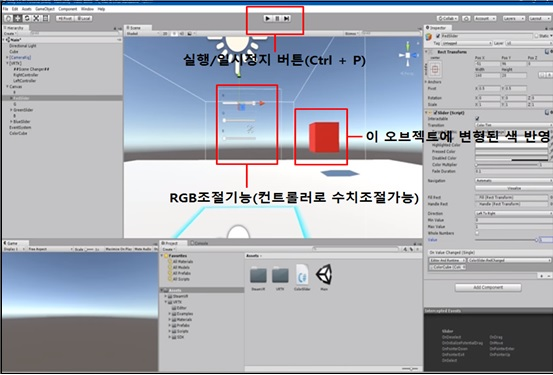
\includegraphics[width=1.0\textwidth]{1-1.jpg}
    \caption{Intro예시}
    \end{figure}
    
    
    \begin{figure}[h!]
    \centering
    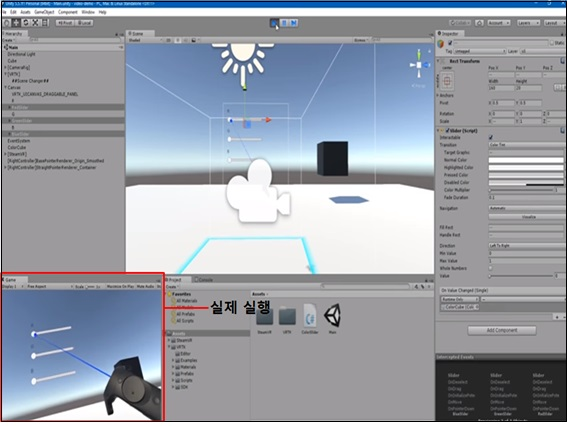
\includegraphics[width=1.0\textwidth]{1-2.jpg}
    \caption{Intro예시}
    \end{figure}
    
    \section{TouchPad Input}
    \subsection{설명}
    
    \begin{itemize}
    

    \item 두번째 예제샘플인 TouchPad Color Picker은 HTC Vive(SteamVR) 기기의 컨트롤러의 터치패드의 좌표값을 받아온후 연산을 하여 HSV 색깔좌표의 값으로 받아와서 RGB색으로 변환하여 오브젝트에 적용을 시킨다. 
    
    \begin{figure}[h!]
    \centering
    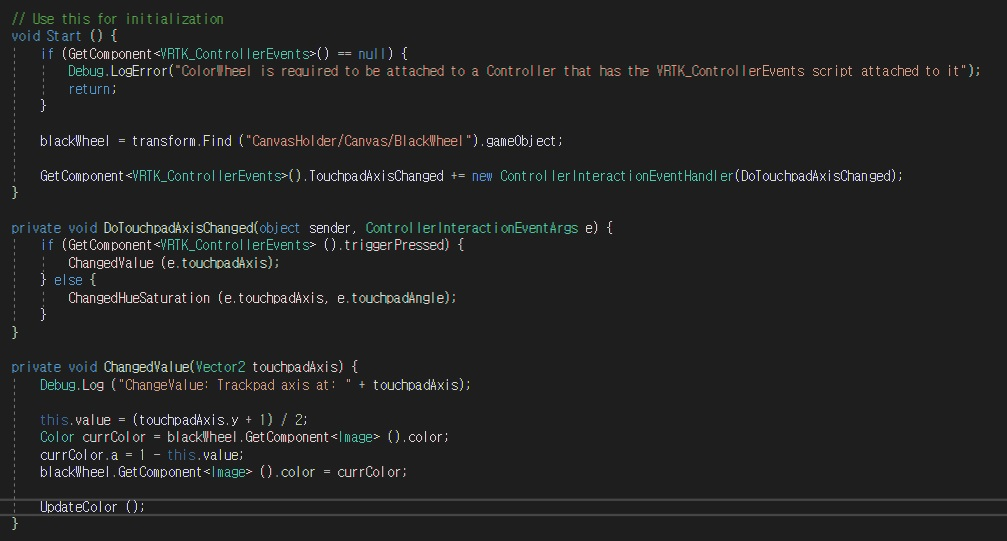
\includegraphics[width=1.0\textwidth]{2-2-1}
    \caption{TouchPad설명}
    \end{figure}
    
    \item VRTK의 컨트롤러 함수를 참조해서 터치패드 좌표 X,Y와 트리거 버튼을 가져온다. 
    
    \begin{figure}[h!]
    \centering
    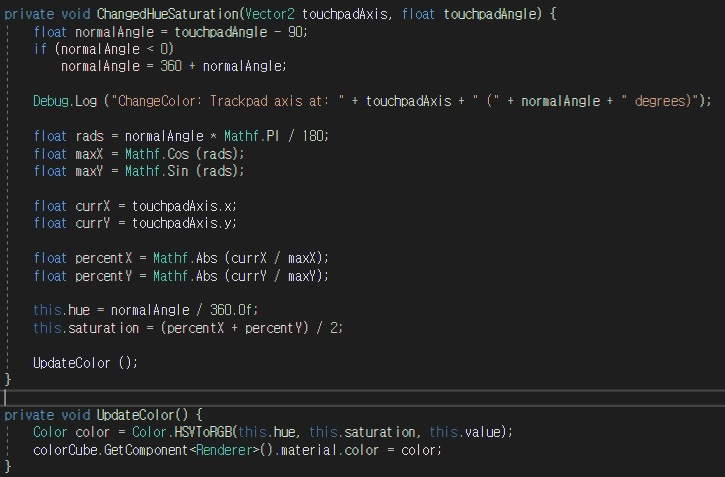
\includegraphics[width=1.0\textwidth]{2-2-1-1.jpg}
    \caption{TouchPad설명}
    \end{figure}
    
   


    \end{itemize}
    
    \subsection{예시}
    
    
    \begin{figure}[h!]
    \centering
    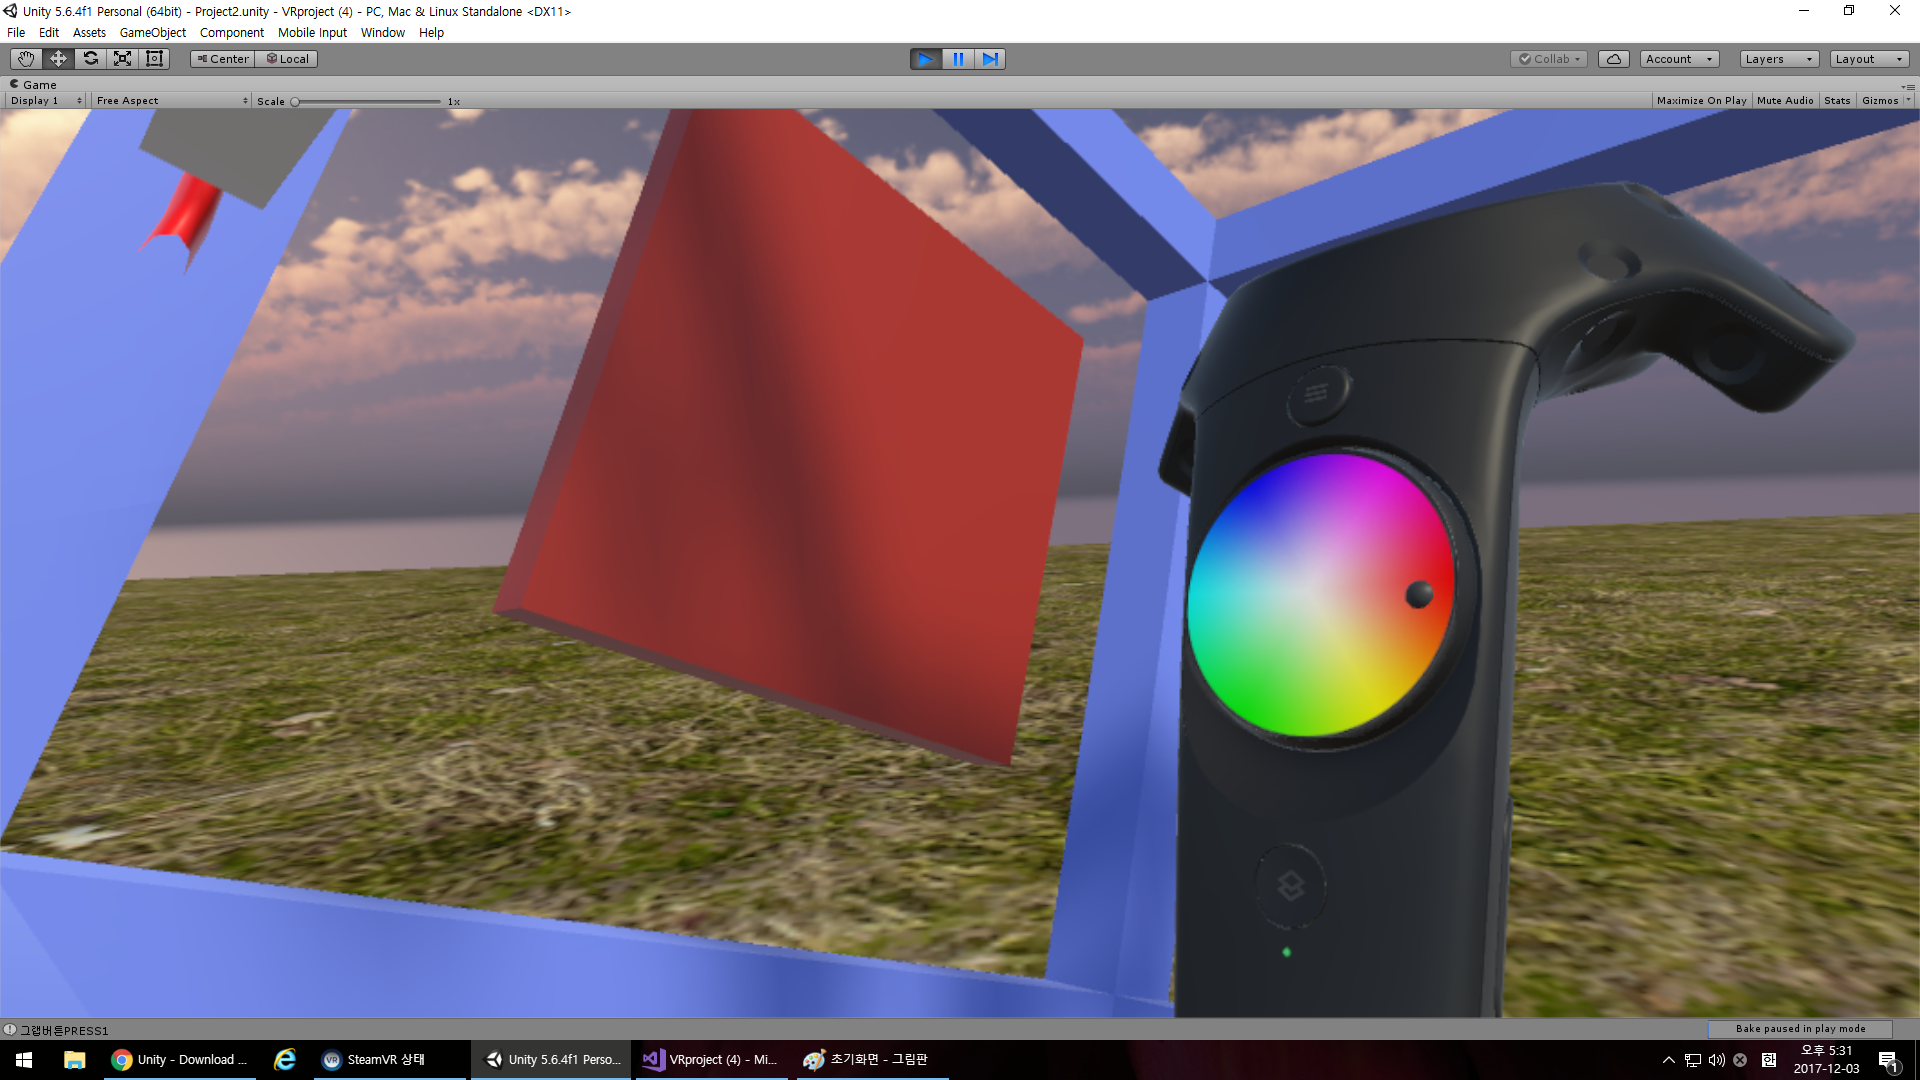
\includegraphics[width=1.0\textwidth]{vrtk2-1.jpg}
    \caption{TouchPad예시}
    \end{figure}
    
    \section{Grab Objects}
    \subsection{설명}
    
    \begin{itemize}
    
    \item 하나의 물체를 오브젝트로 선언.

    \item 레이캐스트와 콜리더를 통해 컨트롤러와 선언한 오브젝트의 충돌을 감지

    \item 충돌 후 컨트롤러 트리거 작동 시, 해당 물체를 컨트롤러로 잡은걸로 선언되어 컨트롤러가 움직이는대로 해당 오브젝트가 따라옴


    

    \end{itemize}
    
    \subsection{예시}
    
    \begin{figure}[h!]
    \centering
    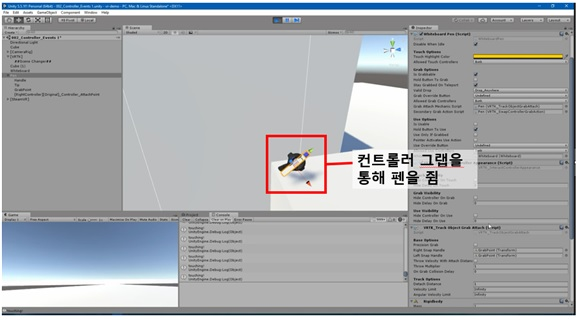
\includegraphics[width=1.0\textwidth]{vrtk3-1.jpg}
    \caption{Grab예시}
    \end{figure}
    
    \begin{figure}[h!]
    \centering
    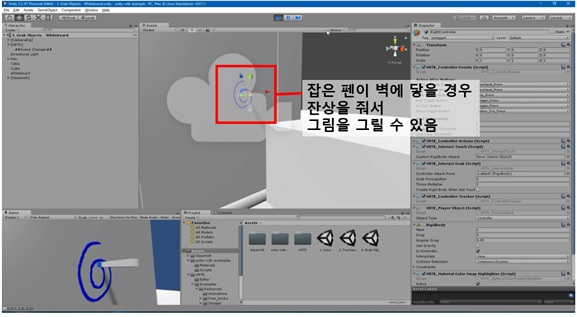
\includegraphics[width=1.0\textwidth]{vrtk3-2.jpg}
    \caption{Grab예시}
    \end{figure}
    

    \section{Gaze UI}
    \subsection{설명}
    
    \begin{itemize}
    
    \item 시선 처리에 따른 UI 설명
    \item 카메라 리그의 자식오브젝트 헤드 / 헤드의 자식오브젝트 아이의 시점을 시선처리로 설정.

    \item 대상은 캔버스 오브젝트의 자식오브젝트 버튼을 생성.
    \item 버튼 자식오브젝트 텍스트 생성 후
    \item 시선이 대상에 닿으면 색상이 변경되는 것을 확인할 수 있다.




    \end{itemize}
    
    \subsection{예시}
    
    \begin{figure}[h!]
    \centering
    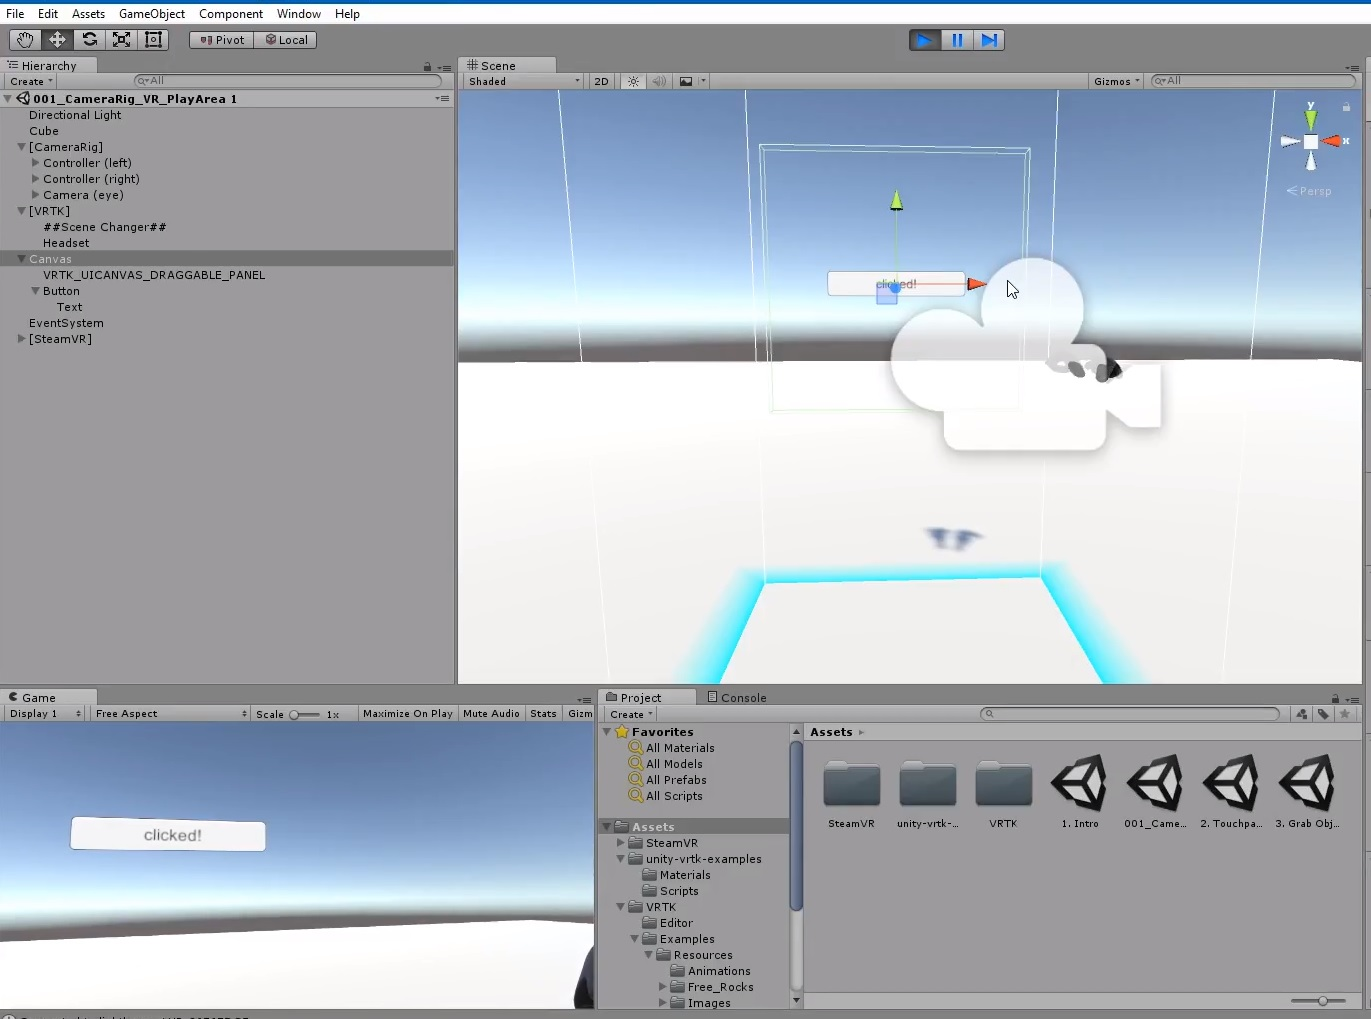
\includegraphics[width=1.0\textwidth]{vrtk4-1.jpg}
    \caption{GazeUI예시}
    \end{figure}
    
 
    
    
    \section{Sword Grab}
    
    \subsection{설명}
    
    \begin{itemize}

    \item 컨트롤러에 SWORD 오브젝트를 붙이고 뗄수 있는 기능
    \item HTC VIVE의 CameraRig에 각각의 left 와 right의 Controller이 기본 prefab으로 있음
    \item VIVE의 CameraRig의 Controller를 VRTK의 Controller로 사용
    \item VRTK의 VRTK Interact Touch와 VRTK Interact Grab을 사용
    \item CreateEmpty 를 생성해서 Headset으로 주고, Transfrom Follow로 주고, Foller를 eye로 설정
    \item Backpack에 OnTriggerStay를 주고, InteractGrabdmf Collider로 줘서 사용
    \item Sword라는 스크립트를 추가하여, 이후 Controller grap시 Sword생성
    \item Grab해제 시 해당 Sword prefab은 rigidbody에 의해 땅으로 떨어지며, 다시 grab시 새로운 sword clone prefab이 생성

    \end{itemize}
    
    \subsection{예시}
    
    \begin{figure}[h!]
    \centering
    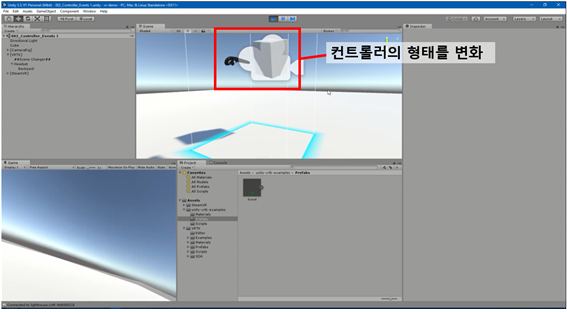
\includegraphics[width=1.0\textwidth]{vrtk5-1.jpg}
    \caption{SwordGrab예시}
    \end{figure}
    
    \begin{figure}[h!]
    \centering
    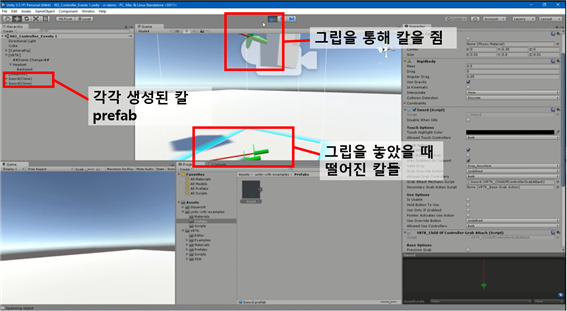
\includegraphics[width=1.0\textwidth]{vrtk5-2.jpg}
    \caption{SwordGrab예시}
    \end{figure}
    
 
    \chapter {오픈소스SW의 버그 및 원인 또는 기능 향상을 위한 제안}
    \section {후기}
    
    \begin{itemize}
    
    \item {20104834 이창수(조장ID)}
    \item [ -]바이브 컨트롤러를 사용한 모델링 작업을 수행할 프로그램을 제작가능할 수 있다.
    \item [ -]이를 통해 멀티플레이어 작업을 연동한다면 다양한 분야의 모델링 작업을 협업할 수 있다.
    \item [ -]ex)의료분야 자동차 디자인분야 건축분야 등등

    
    \item {20124859 박지환(GitHub:genari7)}
    \item [ -]VIVE를 사용하여 프로젝트를 만드는데 있어서 유용한 기능들을 모아놓아서 유용하다.
    \item [ -]연구실을 찾아가서 따라 만든 파일을 직접 시연해보니 좋았다.
    \item [ -]협업을 위한 GITHUB와 레포트를 편하게 만들수 있는 LATEX의 사용법을 공부해보니 앞으로 유용하게 쓰일거 같다.
    
    \item {20134833 김진혁(branch:hoxfix2)}
    \item [ -]SteamVR에서 걸어놓은 제약조건을 쉽게 해결할 수 있었다.
    \item [ -]다양한 프리팹과 예시들이 있어서, 원하는 것을 조금 더 쉽게 제작할 수 있었다.
    \item [ -]VR에서 우리가 생각하는 것보다 다양한 기능을 구현할 수 있었으며, 이와 관련된 여러 작품들이 많이 나와있다는 것을 알 수 있었다.

    \end{itemize}

    

\end{document}



 